\documentclass[12]{report}

%import packages for theoretical computer science stuff
\usepackage{amsmath}
\usepackage{amssymb}
\usepackage{amsthm}
\usepackage{mathrsfs}

%import packages for images
\usepackage{graphicx}
\usepackage{float}

%import packages for algorithms
\usepackage{algorithm}
\usepackage{algorithmic}
\usepackage{listings}
\usepackage{graphicx}

\usepackage{subfigure}
\usepackage{subcaption}
\usepackage{caption}
\usepackage{longtable}


%import packages for automata
\usepackage{tikz}
\usetikzlibrary{automata,positioning}
\usetikzlibrary{graphs,positioning}
\usetikzlibrary{chains,fit,shapes}

%setup document margins and spacing
\usepackage[margin=1in]{geometry}
\usepackage{setspace}
\onehalfspacing


%import packages for hyperlinks
\usepackage{hyperref}
\hypersetup{
    colorlinks=true,
    linkcolor=purple,
    filecolor=magenta,
    urlcolor=cyan,
}


%begin document
\begin{document}

\title{Machine Learning - House Prices Analysis}
%insert 5 members of the group
\author{Daniele Avolio : 242423\\
    \and
    Alessandro Fazio : 242422\\
    \and
    Merem Hassem Indiris\\
    \and
    Michele Vitale\\
    \and
    Lorenzo Piro\\}
\date{A.Y. 2022/2023}
\maketitle


\begin{titlepage}
    %insert a fullpage cover image without considering margins
    \noindent\makebox[\textwidth]{%
        \includegraphics[width=\paperwidth,height=\paperheight]{imgs/project cover.png}
    }
\end{titlepage}

\tableofcontents



\newpage



\chapter{Introduction}
\label{sec:introduction}

To develop this \textbf{Machine Learning} project we are going to use the CRISP-DM methodology, which is a well-known and widely used methodology for data mining projects. It is an iterative process that is composed of six phases.

In particulal, the phases are:
\begin{enumerate}
    \item \textbf{Business Understanding}: in this phase we will try to understand the problem and the objectives of the project. We will also try to understand the data that we have at our disposal and how we can use it to solve the problem.
    \item \textbf{Data Understanding}: in this phase we will try to understand the data that we have at our disposal. We will try to understand the meaning of the data and how we can use it to solve the problem.
    \item \textbf{Data Preparation}: in this phase we will try to prepare the data for the next phases. We will try to clean the data and to transform it in a way that will be useful for the next phases.
    \item \textbf{Modeling}: in this phase we will try to build a model that will be able to solve the problem. We will try to find the best model for our problem.
    \item \textbf{Evaluation}: in this phase we will try to evaluate the model that we have built. We will try to understand if the model is good enough to solve the problem.
    \item \textbf{Deployment}: in this phase we will try to deploy the model that we have built. We will try to understand how we can use the model to solve the problem.
\end{enumerate}

\begin{figure}[H]
    \centering
    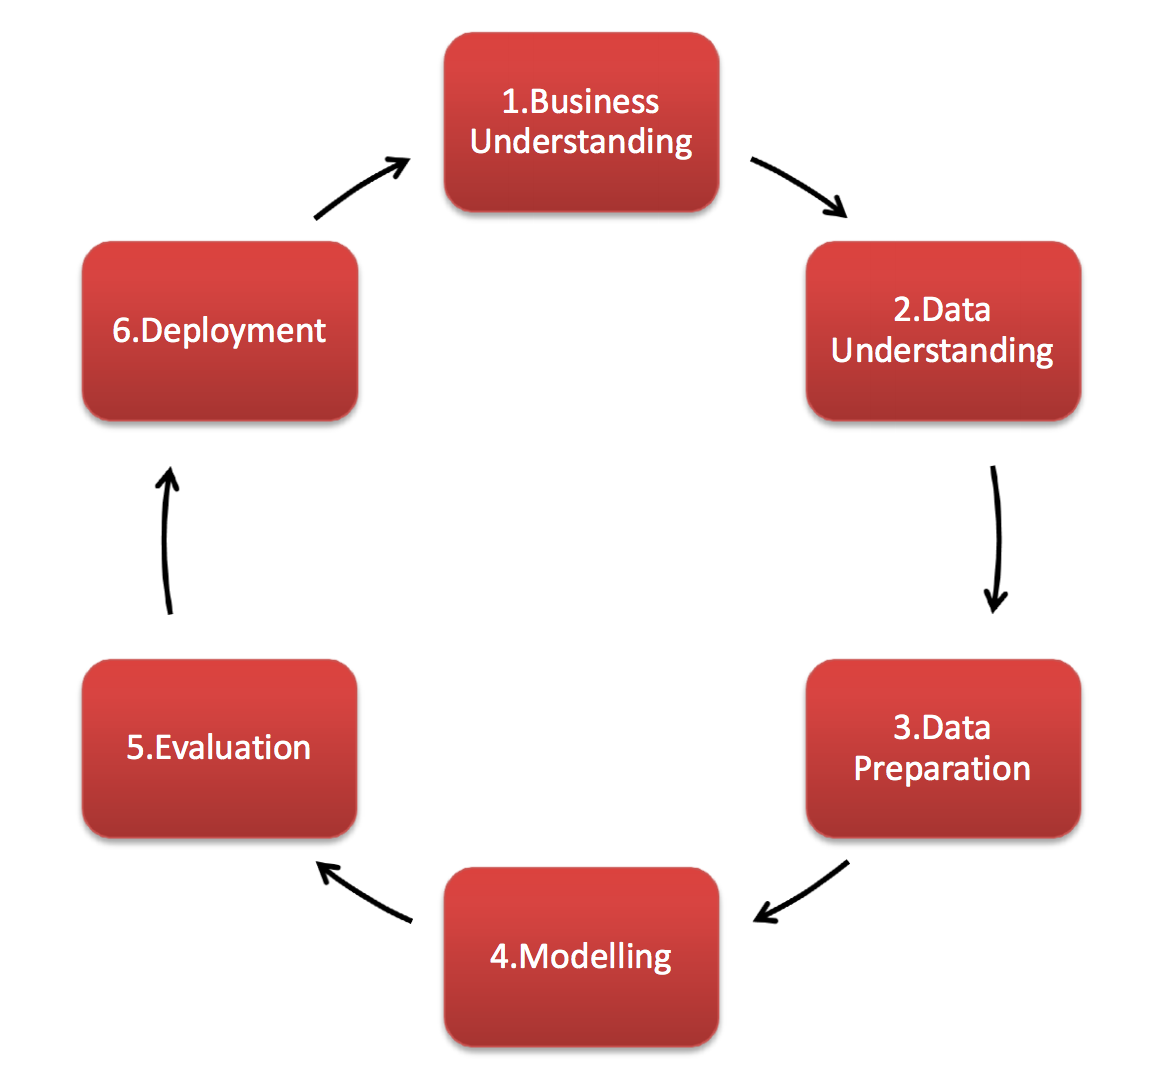
\includegraphics[width=0.5\textwidth]{imgs/crisp.png}
    \caption{CRISP-DM methodology}
    \label{fig:crisp-dm}
\end{figure}
\newpage

\chapter{Business understanding}
\label{sec:business_understanding}

\section{Background}
Our project is based using the dataset of the Kaggle competition \href{https://www.kaggle.com/c/house-prices-advanced-regression-techniques}{House Prices: Advanced Regression Techniques}. 

The goal of the competition is to predict the final price of each home based on 79 explanatory variables describing (almost) every aspect of residential homes in Ames, Iowa.
The dataset is composed by 1460 rows and 81 columns, with an ID column and the last one which is the target variable, the Sale Price.

A small list of the variables is the following:

\begin{itemize}
    \item \textbf{LotArea}: Lot size in square feet
    \item \textbf{OverallQual}: Overall material and finish quality
    \item \textbf{OverallCond}: Overall condition rating
    \item \textbf{YearBuilt}: Original construction date
    \item \textbf{YearRemodAdd}: Remodel date
    \item \textbf{RoofStyle}: Type of roof
    \item \textbf{Exterior1st}: Exterior covering on house
    \item \textbf{Exterior2nd}: Exterior covering on house (if more than one material)
    \item \textbf{MasVnrType}: Masonry veneer type
    \item \textbf{MasVnrArea}: Masonry veneer area in square feet
    \item \dots
\end{itemize}
\section{Business objectives}
\label{subsec:business_objectives}

In this part we are going to analyze the business objective of the project.
Our goal is different from the one of the competition, in fact we are requested to \textbf{convert the Sale Price variable into 3 ranges}:

\begin{enumerate}
    \item \textbf{LOW}: From 0 to 150000 
    \item \textbf{MEDIUM}: From 150000 to 300000 
    \item \textbf{HIGH}: From 300000 and beyond 
\end{enumerate}

So, our goal is to predict a categorical variable with 3 possible values, instead of a continuous variable. 
This is a very important difference, because we are not interested in the exact value of the Sale Price, but only in the range in which it falls.

\section{Business success criteria}
\label{subsec:business_success_criteria}
The success criteria of the project is to obtain a model that is able to predict the Sale Price range with a good accuracy. In particular, we want to create a model that is able to predict the Sale Price range with an accuracy of at least 0.8.

\section{Assessment of the situation}
\label{subsec:assessment_of_the_situation}

There is a very important aspect that we have to consider: there are a lot of variables in the dataset that contains a values of \textbf{NA}, that could leat to thinking that the value is missing.

Actually, this is not always true. In particular, the description of the dataset contains information about the meaning of the \textbf{NA} value for each variable. For example, the \textbf{NA} value for the \textbf{PoolQC} variable means that the house doesn't have a pool, so the value is not missing, but it is a value that has a meaning.

There are more variables that have a similar meaning for the \textbf{NA} value, so we have to be careful when we are going to handle the missing values. For this project, we are going to assume that the \textbf{NA} value is not missing but is just a value that has a meaning. If we need to drop the column, will be specified in the particular section

\section{Inventory of resources}
\label{subsec:inventory_of_resources}

For this project, we are going to use the following resources:

\begin{itemize}
    \item \textbf{Python 3.10.6}: The programming language used for the project
    \item \textbf{Jupyter Notebook}: The IDE used for the project
    \item \textbf{Pandas}: used for data manipulation
    \item \textbf{Numpy}: used for data manipulation
    \item \textbf{Matplotlib}: used for data visualization
    \item \textbf{Seaborn}: used for data visualization
    \item \textbf{Scikit-learn}: used for machine learning 
\end{itemize}

\section{Project Plan}
\label{subsec:project_plan}

The development of the project will be divided into 5 main phases, that are split like this:

%split the phases with duration
\begin{itemize}
    \item \textbf{Phase 1}: Data understanding (1 week)
    \item \textbf{Phase 2}: Data preparation (3 days)
    \item \textbf{Phase 3}: Modeling (1 week)
    \item \textbf{Phase 4}: Evaluation (4 days)
    \item \textbf{Phase 5}: Deployment (none)
\end{itemize}

\newpage



\chapter{Data understanding}
\label{sec:data_understanding}

\section{Data description}
\label{sec:data_description}

The dataset we are using, House Prices - Advanced Regression Techniques, is a dataset containing 79 explanatory variables describing (almost) every aspect of residential homes in Ames, Iowa. The dataset is composed of 1460 rows, each one representing a house, and 81 columns, 80 of which are features and 1 is the target variable, the SalePrice.

With the dataset is provided a \textit{data description} with the description for each variable in thedataset.

%split the table in two parts
\begin{longtable}{|l|p{3cm}|p{4cm}|}
    \caption{Property Features}                                                                                         \\
    \hline
    \textbf{Feature} & \textbf{Description}                                                                             \\
    \hline
    \endfirsthead

    \multicolumn{2}{c}%
    {{\tablename\ \thetable{} -- continued from previous page}}                                                         \\
    \hline
    \textbf{Feature} & \textbf{Description}                                                                             \\
    \hline
    \endhead

    \hline \multicolumn{2}{r}{{Continued on next page}}                                                                 \\ \hline
    \endfoot

    \hline
    \endlastfoot
    \hline

    \hline
    SalePrice        & The property's sale price in dollars. This is the target variable that you're trying to predict. \\
    \hline
    MSSubClass       & The building class                                                                               \\
    \hline
    MSZoning         & The general zoning classification                                                                \\
    \hline
    LotFrontage      & Linear feet of street connected to property                                                      \\
    \hline
    LotArea          & Lot size in square feet                                                                          \\
    \hline
    Street           & Type of road access                                                                              \\
    \hline
    Alley            & Type of alley access                                                                             \\
    \hline
    LotShape         & General shape of property                                                                        \\
    \hline
    LandContour      & Flatness of the property                                                                         \\
    \hline
    Utilities        & Type of utilities available                                                                      \\
    \hline
    LotConfig        & Lot configuration                                                                                \\
    \hline
    LandSlope        & Slope of property                                                                                \\
    \hline
    Neighborhood     & Physical locations within Ames city limits                                                       \\
    \hline
    Condition1       & Proximity to main road or railroad                                                               \\
    \hline
    Condition2       & Proximity to main road or railroad (if a second is present)                                      \\
    \hline
    BldgType         & Type of dwelling                                                                                 \\
    \hline
    HouseStyle       & Style of dwelling                                                                                \\
    \hline
    OverallQual      & Overall material and finish quality                                                              \\
    \hline
    OverallCond      & Overall condition rating                                                                         \\
    \hline
    YearBuilt        & Original construction date                                                                       \\
    \hline
    YearRemodAdd     & Remodel date                                                                                     \\
    \hline
    RoofStyle        & Type of roof                                                                                     \\
    \hline
    RoofMatl         & Roof material                                                                                    \\
    \hline
    Exterior1st      & Exterior covering on house                                                                       \\
    \hline
    Exterior2nd      & Exterior covering on house (if more than one material)                                           \\
    \hline
    MasVnrType       & Masonry veneer type                                                                              \\
    \hline
    MasVnrArea       & Masonry veneer area in square feet                                                               \\
    \hline
    ExterQual        & Exterior material quality                                                                        \\
    \hline
    ExterCond        & Present condition of the material on the exterior                                                \\
    \hline
    Foundation       & Type of foundation                                                                               \\
    \hline
    BsmtQual         & Height of the basement                                                                           \\
    \hline
    BsmtCond         & General condition of the basement                                                                \\
    \hline
    BsmtExposure     & Walkout or garden level basement walls                                                           \\
    \hline
    BsmtFinType1     & Quality of basement finished area                                                                \\
    \hline
    BsmtFinSF1       & Type 1 finished square feet                                                                      \\
    \hline
    BsmtFinType2     & Quality of second finished area (if present)                                                     \\
    \hline
    BsmtFinSF2       & Type 2 finished square feet                                                                      \\
    \hline
    BsmtUnfSF        & Unfinished square feet of basement area                                                          \\
    \hline
    TotalBsmtSF      & Total square feet of basement area                                                               \\
    \hline
    Heating          & Type of heating                                                                                  \\
    \hline
    HeatingQC        & Heating quality and condition                                                                    \\
    \hline
    CentralAir       & Central air conditioning                                                                         \\
    \hline
    Electrical       & Electrical system                                                                                \\
    \hline
    1stFlrSF         & First Floor square feet                                                                          \\
    \hline
    2ndFlrSF         & Second floor square feet                                                                         \\
    \hline
    LowQualFinSF     & Low quality finished square feet (all floors)                                                    \\
    \hline
    GrLivArea        & Above grade (ground) living area square feet                                                     \\
    \hline
    BsmtFullBath     & Basement full bathrooms                                                                          \\
    \hline
    BsmtHalfBath     & Basement half bathrooms                                                                          \\
    \hline
    FullBath         & Full bathrooms above grade                                                                       \\
    \hline
    HalfBath         & Half baths above grade                                                                           \\
    \hline
    Bedroom          & Number of bedrooms above basement level                                                          \\
    \hline
    Kitchen          & Number of kitchens                                                                               \\
    \hline
    KitchenQual      & Kitchen quality                                                                                  \\
    \hline
    TotRmsAbvGrd     & Total rooms above grade (does not include bathrooms)                                             \\
    \hline
    Functional       & Home functionality rating                                                                        \\
    \hline
    Fireplaces       & Number of fireplaces                                                                             \\
    \hline
    FireplaceQu      & Fireplace quality                                                                                \\
    \hline
    GarageType       & Garage location                                                                                  \\
    \hline
    GarageYrBlt      & Year garage was built                                                                            \\
    \hline
    GarageFinish     & Interior finish of the garage                                                                    \\
    \hline
    GarageCars       & Size of garage in car capacity                                                                   \\
    \hline
    GarageArea       & Size of garage in square feet                                                                    \\
    \hline
    GarageQual       & Garage quality                                                                                   \\
    \hline
    GarageCond       & Garage condition                                                                                 \\
    \hline
    PavedDrive       & Paved driveway                                                                                   \\
    \hline
    WoodDeckSF       & Wood deck area in square feet                                                                    \\
    \hline
    OpenPorchSF      & Open porch area in square feet                                                                   \\
    \hline
    EnclosedPorch    & Enclosed porch area in square feet                                                               \\
    \hline
    3SsnPorch        & Three season porch area in square feet                                                           \\
    \hline
    ScreenPorch      & Screen porch area in square feet                                                                 \\
    \hline
    PoolArea         & Pool area in square feet                                                                         \\
    \hline
    PoolQC           & Pool quality                                                                                     \\
    \hline
    Fence            & Fence quality                                                                                    \\
    \hline
    MiscFeature      & Miscellaneous feature not covered in other categories                                            \\
    \hline
    MiscVal          & \$Value of miscellaneous feature                                                                 \\
    \hline
    MoSold           & Month Sold                                                                                       \\
    \hline
    YrSold           & Year Sold                                                                                        \\
    \hline
    SaleType         & Type of sale                                                                                     \\
    \hline
    SaleCondition    & Condition of sale                                                                                \\
\end{longtable}


An important thing to specify is that the dataset is given with an additional "data\_description.txt" file that describes the features in detail. This file is used to understand the features and their values. From here, some
variables have a specific value to point the fact the the house doesn't have that feature. For example, the feature "Alley" has the value "NA" to point the fact that the house doesn't have an alley. This is important to know.
The next list contains all the features that have the value 'NA' indicating the non-existence of the feature.
\begin{enumerate}
    \item Alley
    \item BsmtQual
    \item BsmtCond
    \item BsmtExposure
    \item BsmtFinType1
    \item BsmtFinType2
    \item FireplaceQu
    \item GarageType
    \item GarageFinish
    \item GarageQual
    \item GarageCond
    \item PoolQC
    \item Fence
    \item MiscFeature
\end{enumerate}

In this project, as a team we decided to consider those variables \textbf{not null}, and considering the value 'NA' always as the non-existence of the feature. This is important to know because it will be used in the data cleaning phase.

Note that this is not related to the other variables, since the variables not mentioned in the above list have the value 'NA' to indicate \textbf{null value}. For example, if in some rows the feature "MasVnrType" has the value "NA", it means that the value is null and not that the house doesn't have a masonry veneer type.

\textbf{If something is missing please fill this section.}

\section{Data exploration}
\label{sec:data_exploration}

The dataset contains 81 features, and 1460 rows. The attributes gives information about the house, and the target variable is the SalePrice. The goal of this project is to predict the SalePrice of a house given the features. The features are a mix of categorical and numerical variables.
\begin{figure}[h!]
    \centering
    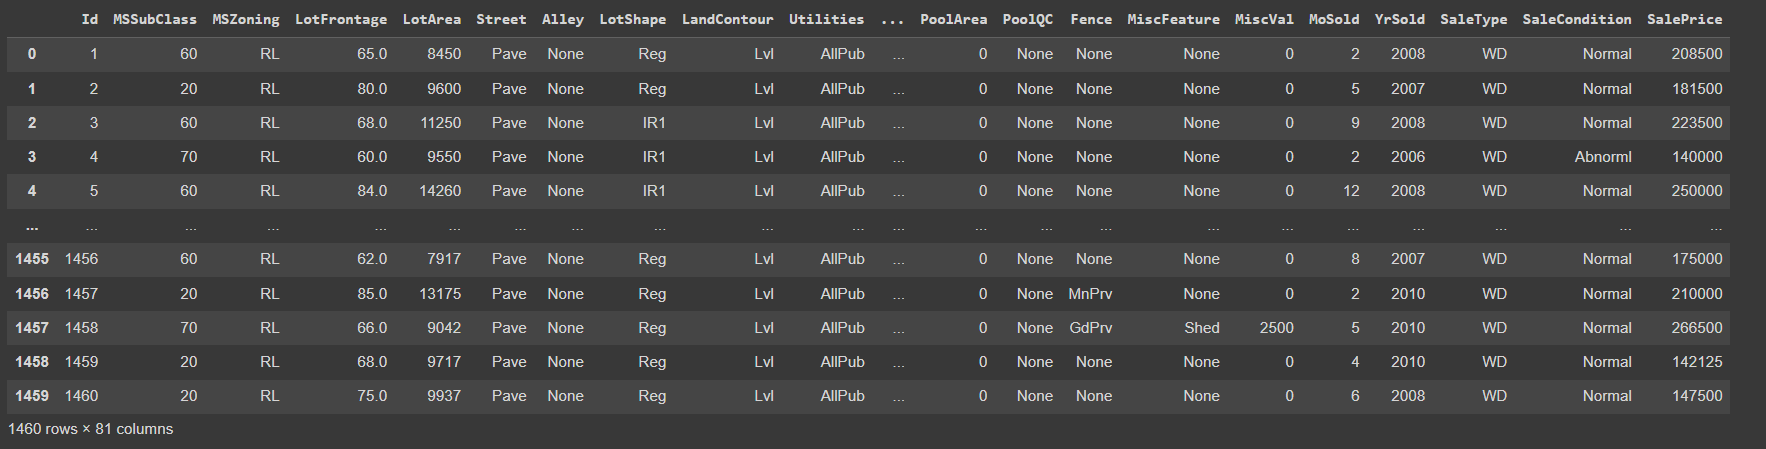
\includegraphics[width=0.8\textwidth]{imgs/desc1.png}
    \caption{Dataset print}
    \label{fig:dataset_print}
\end{figure}

\begin{lstlisting}
<class 'pandas.core.frame.DataFrame'>
RangeIndex: 1460 entries, 0 to 1459
    Data columns (total 81 columns):
    #   Column         Non-Null Count  Dtype  
    ---  ------         --------------  -----  
    0   Id             1460 non-null   int64  
    1   MSSubClass     1460 non-null   int64  
    2   MSZoning       1460 non-null   object 
    3   LotFrontage    1201 non-null   float64
    4   LotArea        1460 non-null   int64  
    5   Street         1460 non-null   object 
    6   Alley          91 non-null     object 
    7   LotShape       1460 non-null   object 
    8   LandContour    1460 non-null   object 
    9   Utilities      1460 non-null   object 
    10  LotConfig      1460 non-null   object 
    11  LandSlope      1460 non-null   object 
    12  Neighborhood   1460 non-null   object 
    13  Condition1     1460 non-null   object 
    14  Condition2     1460 non-null   object 
    15  BldgType       1460 non-null   object 
    16  HouseStyle     1460 non-null   object 
    17  OverallQual    1460 non-null   int64  
    18  OverallCond    1460 non-null   int64  
    19  YearBuilt      1460 non-null   int64  
    20  YearRemodAdd   1460 non-null   int64  
    21  RoofStyle      1460 non-null   object 
    22  RoofMatl       1460 non-null   object 
    23  Exterior1st    1460 non-null   object 
    24  Exterior2nd    1460 non-null   object 
    25  MasVnrType     588 non-null    object 
    26  MasVnrArea     1452 non-null   float64
    27  ExterQual      1460 non-null   object 
    28  ExterCond      1460 non-null   object 
    29  Foundation     1460 non-null   object 
    30  BsmtQual       1423 non-null   object 
    31  BsmtCond       1423 non-null   object 
    32  BsmtExposure   1422 non-null   object 
    33  BsmtFinType1   1423 non-null   object 
    34  BsmtFinSF1     1460 non-null   int64  
    35  BsmtFinType2   1422 non-null   object 
    36  BsmtFinSF2     1460 non-null   int64  
    37  BsmtUnfSF      1460 non-null   int64  
    38  TotalBsmtSF    1460 non-null   int64  
    39  Heating        1460 non-null   object 
    40  HeatingQC      1460 non-null   object 
    41  CentralAir     1460 non-null   object 
    42  Electrical     1459 non-null   object 
    43  1stFlrSF       1460 non-null   int64  
    44  2ndFlrSF       1460 non-null   int64  
    45  LowQualFinSF   1460 non-null   int64  
    46  GrLivArea      1460 non-null   int64  
    47  BsmtFullBath   1460 non-null   int64  
    48  BsmtHalfBath   1460 non-null   int64  
    49  FullBath       1460 non-null   int64  
    50  HalfBath       1460 non-null   int64  
    51  BedroomAbvGr   1460 non-null   int64  
    52  KitchenAbvGr   1460 non-null   int64  
    53  KitchenQual    1460 non-null   object 
    54  TotRmsAbvGrd   1460 non-null   int64  
    55  Functional     1460 non-null   object 
    56  Fireplaces     1460 non-null   int64  
    57  FireplaceQu    770 non-null    object 
    58  GarageType     1379 non-null   object 
    59  GarageYrBlt    1379 non-null   float64
    60  GarageFinish   1379 non-null   object 
    61  GarageCars     1460 non-null   int64  
    62  GarageArea     1460 non-null   int64  
    63  GarageQual     1379 non-null   object 
    64  GarageCond     1379 non-null   object 
    65  PavedDrive     1460 non-null   object 
    66  WoodDeckSF     1460 non-null   int64  
    67  OpenPorchSF    1460 non-null   int64  
    68  EnclosedPorch  1460 non-null   int64  
    69  3SsnPorch      1460 non-null   int64  
    70  ScreenPorch    1460 non-null   int64  
    71  PoolArea       1460 non-null   int64  
    72  PoolQC         7 non-null      object 
    73  Fence          281 non-null    object 
    74  MiscFeature    54 non-null     object 
    75  MiscVal        1460 non-null   int64  
    76  MoSold         1460 non-null   int64  
    77  YrSold         1460 non-null   int64  
    78  SaleType       1460 non-null   object 
    79  SaleCondition  1460 non-null   object 
    80  SalePrice      1460 non-null   int64  
dtypes: float64(3), int64(35), object(43)
memory usage: 924.0+ KB
\end{lstlisting}

\subsection{Preliminary operation on data preparation}
\label{sec:preliminary_operation_on_data_preparation}

In order to achieve \textbf{better results looking at data and graphs}, we decided to
do some data transformation and cleaning before the data processing part. This choice brings 
an easier and more intuitive data visualization and analysis for us, in order to get a better
insight of the data. 

The action carried out in this part are the following:
\begin{enumerate}
    \item Trasnforming \textbf{NA} values into \textbf{no\_value} for the categorical features written in the precedent section.
    \item Setting GarageYrBlt, MasVnrArea, LotFrontage null values to \textbf{0}
    \item Changing all the columns with attribute \textbf{object} to \textbf{category} type
    \item Changed MasVnrArea and LotFrontage to \textbf{int64} type
    \item Dropped one row with Electrical null value
    \item Others changes during data visualization part (Will be reported in the data processing section)   
\end{enumerate}

\subsection{Data Exploration - More in depth}
\label{sec:data_exploration_more_in_depth}

%insert 2 images in one row

\begin{figure}[h!]
    \centering
    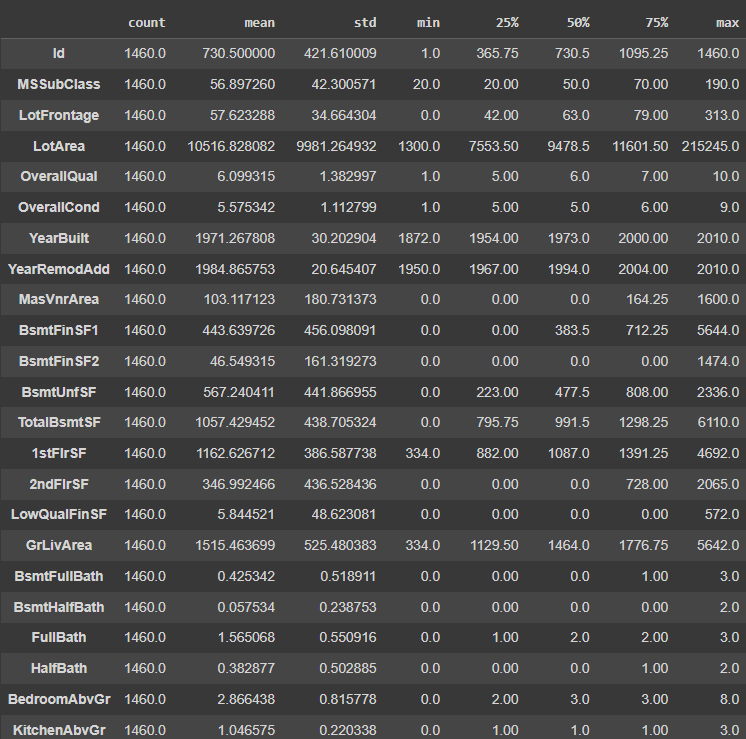
\includegraphics[width=0.8\textwidth]{imgs/info1.png}
    \caption{Numerical info 1}
    \label{fig:info1}
\end{figure}

\begin{figure}[h!]
    \centering
    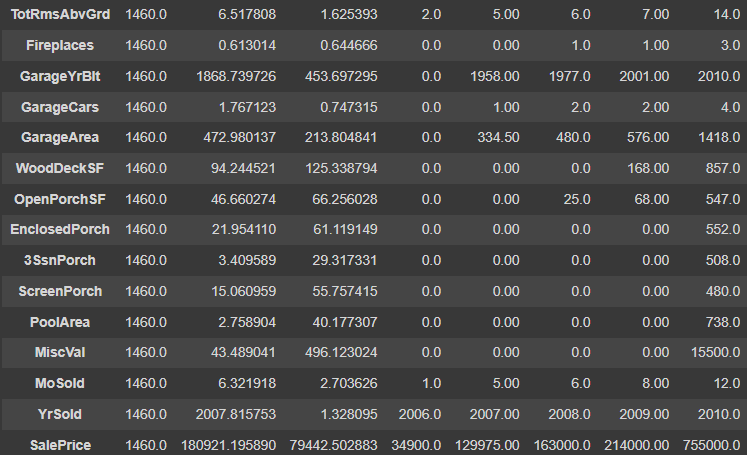
\includegraphics[width=0.8\textwidth]{imgs/info2.png}
    \caption{Numerical info 2}
    \label{fig:info2}
\end{figure}

\begin{figure}[h!]
    \centering
    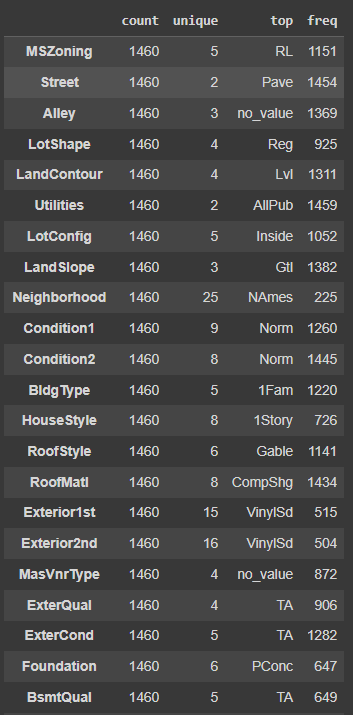
\includegraphics[width=0.8\textwidth]{imgs/info3.png}
    \caption{Categorical info 1}
    \label{fig:info3}
\end{figure}

\begin{figure}[h!]
    \centering
    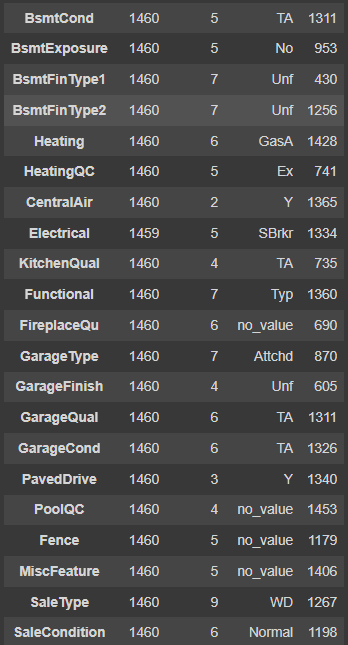
\includegraphics[width=0.8\textwidth]{imgs/info4.png}
    \caption{Categorical info 2}
    \label{fig:info4}
\end{figure}

\end{document}
